\documentclass[11pt,a4paper]{article}
\usepackage[T1]{fontenc}
\usepackage[margin=25mm,headheight=14pt]{geometry}
\usepackage{amsmath,booktabs,graphicx,float,fancyhdr,siunitx}
\usepackage[american]{circuitikz}
\usepackage[hidelinks]{hyperref}
\setlength{\parskip}{.55\baselineskip}\setlength{\parindent}{0pt}
\pagestyle{fancy}\fancyhf{}
\fancyhead[R]{Adam Omarali and Jin Hongjun}\fancyfoot[C]{\thepage}
\begin{document}
\hypersetup{pageanchor=false}
\begin{titlepage}\centering
\vspace*{1cm}
\includegraphics[height=3.8cm]{figure-1.png}\par\vspace{1cm}
{\Large ETIN71\par}{\large Introduction to Integrated Electronics\par}\vfill
{\Huge\bfseries Design and Evaluation of a Nanowire CMOS Differential Amplifier\par}\vspace{1cm}
{\Large Project Report\par}\vfill{\large Adam Omarali\\Jin Hongjun\par}\vfill
{\large 6 October 2026\par}
\end{titlepage}
\hypersetup{pageanchor=true}
\pagenumbering{arabic}

\section{Introduction}

This report details the design, simulation and evaluation of a two-stage differential amplifier shown in Figure~\ref{fig:diffamp}. The circuit was designed in Qucs~\cite{qucs} using nanowire (NW) MOSFET models. These complementary NW CMOS devices feature a gate-all-around geometry and utilize III-V materials (such as InAs) to achieve higher carrier mobility and improved electrostatics compared to traditional planar transistors~\cite{brief}. Because their behavior is decoupled from traditional area scaling, they can be accurately modeled and evaluated much like standard short-channel MOSFETs.

Throughout this project, the provided Nanoelectronics Student Component Library (NSCL) was used to construct and systematically evaluate a complete analog amplifier circuit. The design from Figure~\ref{fig:diffamp} incorporates an NMOS differential input pair ($Q_1$, $Q_2$), a PMOS current mirror active load ($Q_3, Q_4$), a current steering bias network ($Q_6, Q_7, Q_8$), and a common-drain output stage ($Q_5$) acting as a voltage follower. By iteratively tuning component geometries through DC bias configurations and evaluating the frequency response via AC simulations, the project aimed to verify the real-world capabilities of the NW MOSFET technology and compare the resulting circuit's performance against the theoretical characteristics of an ideal operational amplifier (op-amp).

\begin{figure}[H]\centering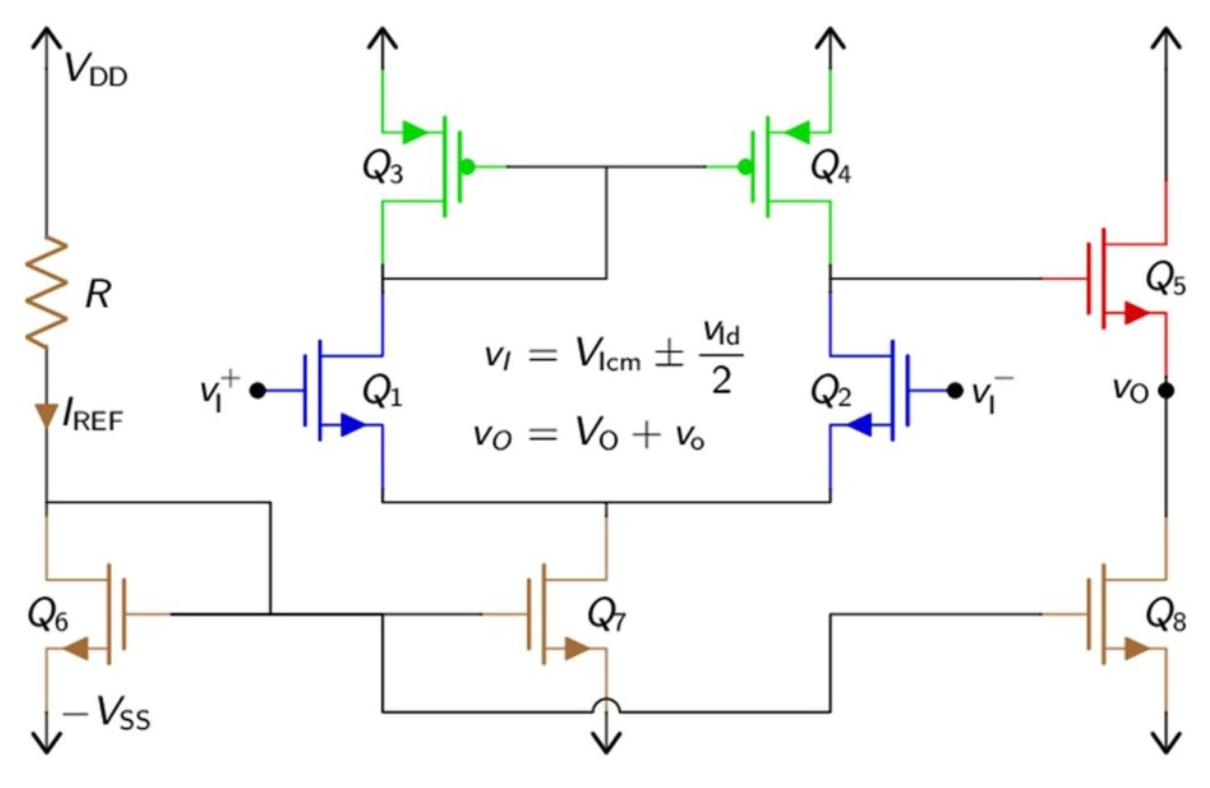
\includegraphics[width=.6\linewidth]{figure-3.png}
\caption{Differential Amplifier provided by the lab manual~\cite{brief} comprised of an NMOS differential input (blue), PMOS current mirror load (green), NMOS current steering bias (yellow) and an NMOS common drain output (red).}
\label{fig:diffamp}\end{figure}

\section{Theory}

This section will explore the characteristics of an ideal op-amp, the important MOSFET parameters related to these ideal characteristics, and MOSFET configurations used in our amplifier design.
\subsection{Ideal Operational Amplifier Characteristics}

An op-amp takes two voltage inputs, one non-inverting, ${v}_{i}^+$, and one inverting, ${v}_{i}^-$, amplifies their difference, and outputs a voltage to be used by the remaining circuit, ${v}_{o}$. The relationship between the differential inputs and output voltage is given by:

\begin{equation}
    v_o = A_{OL}(v_{i}^+ - v_{i}^-)
    \label{eq:open-loop-gain}
\end{equation}

where $A_{OL}$ is the open loop amplifier gain, which determines how effectively the op-amp increases the signal. An open loop (OL) op-amp has no feedback connection from its output to either input. For an ideal OL op-amp, ${A}_{OL}=\infty$. 

The ideal op-amp also assumes infinite input impedance ${R}_{in}=\infty$ so that no current is drawn by the input terminals and therefore the op-amp does not load the signal source. Similarly we assume ${R}_{out}=0$ so the output voltage is unaffected by the current drawn by the load. 

For equal input voltages, the differential input is zero, and therefore we expect $v_{o}=0$. This is not always the case due to internal device mismatching.

Another common property is gain performance across frequencies. The upper cutoff frequency is the frequency at which the low frequency gain decreases by 3 dB. For this low-pass response, the bandwidth ($BW$) extends from DC to the upper cutoff frequency. For an ideal op-amp with no capacitive effects, $BW=\infty$.

A voltage follower is a closed loop (CL) configuration, where the output voltage is connected directly to the inverting input resulting in $v_o = v_i^-$. Plugging this condition into Equation~\eqref{eq:open-loop-gain} we can find the closed loop gain, $A_{CL}$:
\begin{align}
    v_o &= A_{OL}\left(v_i^+ - v_o\right) \notag \\
    v_o\left(1 + A_{OL}\right) &= A_{OL}v_i^+ \notag \\
    A_{CL}
        &= \frac{v_o}{v_i^+}
        = \frac{A_{OL}}{1 + A_{OL}}
    \label{eq:closed-loop-gain}
\end{align}

As $A_{OL}$ approaches infinity, $A_{CL}$ approaches 1. This is called the voltage follower configuration since $v_o$ approaches $v_i^+$ as $A_{OL}$ increases.
\subsection{Nanowire MOSFET Large \& Small Signal Models}

A MOSFET is a voltage-controlled current source, whereby supplying specific voltages to each of its three terminals (drain, gate, source), we can influence the drain current, ${I}_{D}$, and its mode of operation. For amplifier design, we want all MOSFETs to operate in saturation. For an NMOS transistor, this is satisfied by the conditions:
\begin{equation}
    V_{GS}>V_t, \qquad V_{DS} \geq V_{GS} - V_t
    \label{eq:saturation-condition}
\end{equation}

For a PMOS transistor, the analogous conditions are expressed using $V_{SG}$, $V_{SD}$ and $|V_{tp}|$.

The $I_D$ relationship for a MOSFET in saturation is approximately given by:
\begin{equation}
    {I}_{D}=\frac{1}{2}{k}_{n}'\frac{W}{L}({V}_{GS}-{V}_{t})^{2}(1 + \lambda V_{DS})
    \label{eq:mosfet-current}
\end{equation}
where ${k}_{n}'$ is a material parameter, $\frac{W}{L}$ is the width-to-channel-length ratio, ${V}_{GS}$ is the potential difference between the gate and source terminals, ${V}_{t}$ is the threshold voltage where a channel begins to form and the $1 + \lambda V_{DS}$ describes channel length modulation. 
This is an approximation since the NSCL MOSFET performance depends on operating points and other short-channel effects~\cite{brief}.
For the nanowire MOSFETs, $W$ is determined by the following relation with $W_{\mathrm{eq}} = 100\,\mathrm{nm}$ and $NW$ being the number of nanowires, the parameter we used to design our amplifier:

\begin{equation}
W = W_{\mathrm{eq}}NW
\label{eq:nanowire-width}
\end{equation}

For our analysis, we consider a DC voltage operating point $Q$ and small variations about $Q$. The small-signal change in current, $\Delta i_{d}$, due to a small gate-source voltage change, $\Delta v_{gs}$, can be described by a linear small-signal model shown in Figure~\ref{fig:mosfet-model} and by Equation~\eqref{eq:transconductance}.
\begin{figure}[H]
\centering
\begin{circuitikz}[american currents]
    \draw
        (0,2) node[left] {$G$} node[circ] {} coordinate (G)
        (0,0) node[left] {$S$} node[circ] {} coordinate (S)
        (G) -- (1.6,2)
        (S) -- (6.6,0);
    \draw
        (3.5,2) -- (6.6,2)
        (3.5,2) to[cisource] (3.5,0)
        (5.5,2) to[R,l=$r_o$] (5.5,0);
    \draw (3.5,1) node[right=15pt] {$g_m v_{gs}$};
    \draw (6.6,2) node[circ] {} node[right] {$D$};
    \draw (6.6,0) node[circ] {};
    \draw (G) ++(-0.45,-0.25) node {$+$}
          (S) ++(-0.45,0.25) node {$-$}
          ($(G)!0.5!(S)$) ++(-0.75,0) node {$v_{gs}$};
\end{circuitikz}
\caption{Simplified small-signal model of an NMOS transistor}
\label{fig:mosfet-model}
\end{figure}
\begin{equation}
    {\Delta i}_{d|Q} = {g}_{m}{\Delta v}_{gs|Q}
    \label{eq:small-signal-current-change}
\end{equation}
\begin{equation}
    g_m = \left.\frac{\partial I_D}{\partial V_{GS}}\right|_Q
    \label{eq:transconductance}
\end{equation}

where ${g}_{m}$ is the transconductance determined by material properties and DC operating point values. This shows that a small change in the gate-source voltage produces a proportional small-signal change in the drain current, resembling an amplifier.

In Figure~\ref{fig:mosfet-model}, notice there is also an output resistance ${r}_{o}$. This comes from channel length modulation. As $V_{DS}$ increases while the MOSFET remains in saturation, $I_D$ also increases slightly.
\begin{equation}
    {r}_{o}=\left.\frac{\partial {V}_{DS}}{\partial {I}_{D}}\right|_{V_{GS},Q}
    =\left(\left.\frac{\partial I_D}{\partial V_{DS}}\right|_{V_{GS},Q}\right)^{-1}
    \label{eq:output-resistance}
\end{equation}

In a common-source stage, the small-signal drain current produces an output voltage $\Delta v_o=-\Delta i_d r_o$. Combining this with Equation~\eqref{eq:small-signal-current-change} gives the intrinsic voltage gain
\begin{equation}
    A_{v,\mathrm{int}}=\frac{\Delta v_o}{\Delta v_{gs}}
    \approx-g_mr_o, \qquad
    |A_{v,\mathrm{int}}|\approx g_mr_o.
    \label{eq:intrinsic-voltage-gain}
\end{equation}

Using the saturation model in Equation~\eqref{eq:mosfet-current}, $g_m$ and $r_o$ can be approximated by
\begin{equation}
    g_m\approx\frac{2I_D}{V_{OV}}, \qquad
    r_o\approx\frac{1}{\lambda I_D},
    \qquad V_{OV}=V_{GS}-V_t.
    \label{eq:gm-ro-current}
\end{equation}
For a fixed transistor size, $I_D\propto V_{OV}^2$, giving
\begin{equation}
    g_m\propto\sqrt{I_D}, \qquad
    r_o\propto\frac{1}{I_D}, \qquad
    g_mr_o\propto\frac{1}{\sqrt{I_D}}.
    \label{eq:intrinsic-gain-current}
\end{equation}
These relationships are approximations for the short-channel NSCL devices but show how increasing drain current can increase $g_m$ while reducing $r_o$ and intrinsic gain.

\subsection{Amplifier Building Blocks}

\subsubsection{Current Steering}

$Q_6$, $Q_7$ and $Q_8$ form a current mirror that establishes the amplifier bias currents. $Q_6$ is diode connected ($V_G = V_D$) and carries $I_{REF}$. Since $Q_7$ and $Q_8$ share its gate voltage and channel length, using Equation~\ref{eq:mosfet-current}, their currents are approximately scaled by their number of nanowires:
\begin{equation}
    \frac{I_{D7}}{I_{REF}}\approx\frac{NW_7}{NW_6}, \qquad
    \frac{I_{D8}}{I_{REF}}\approx\frac{NW_8}{NW_6}.
    \label{eq:current-mirror-scaling}
\end{equation}
$Q_7$ supplies the differential-pair tail current, while $Q_8$ biases the output stage. The scaling is approximate because unequal $V_{DS}$ values and finite output resistance affect the mirrored currents.

\subsubsection{Differential Pair}

$Q_1$ and $Q_2$ form an NMOS differential pair driven by $v_{id}=v_i^+-v_i^-$. 
When $v_{id}=0$, matched devices divide the $Q_7$ tail current approximately equally, so $I_{D1}\approx I_{D2}\approx I_{D7}/2$. 
For a small positive $v_{id}$, $I_{D1}$ increases and $I_{D2}$ decreases by Equation~\ref{eq:small-signal-current-change}. 
\begin{equation}
\begin{aligned}
\Delta i_{d1} &= +\frac{g_m}{2}\Delta v_{id},
\qquad
\Delta i_{d2} &= -\frac{g_m}{2}\Delta v_{id}.
\label{eq:differential-current-change}
\end{aligned}
\end{equation}
The stage therefore converts the differential input voltage into opposing drain-current changes.

\subsubsection{Current Mirror Load}

$Q_3$ and $Q_4$ form a PMOS current-mirror active load. $Q_3$ is diode connected, and $Q_4$ approximately mirrors its current into the $Q_2$/$Q_4$ node. When $v_i^+$ increases relative to $v_i^-$, $Q_4$ mirrors the increased $Q_1$ current described by Equation~\ref{eq:differential-current-change} into the output-side branch. 
Together, $Q_1$--$Q_4$ form the first gain stage. The resistance at the shared drain node of $Q_2$ and $Q_4$ is approximately $r_{o2}\parallel r_{o4}$, which is a high resistance because both transistors operate in saturation. The mirror converts the differential current into a voltage with a gain $A_{v1}$:
\begin{equation}
    A_{v1}\approx g_m\left(r_{o2}\parallel r_{o4}\right).
    \label{eq:first-stage-gain}
\end{equation}

where $g_m$ is the transconductance of $Q_1/Q_2$ assuming matching.

\subsubsection{Common Drain Output Stage}

$Q_5$ is a common-drain amplifier, or source follower, driven by the output of the first gain stage and biased by the $Q_8$ current sink. The small-signal resistance at its source is approximately $R_S=r_{o5}\parallel r_{o8}$. Neglecting body effect, its voltage gain is
\begin{equation}
    A_{v2}\approx\frac{g_{m5}R_S}{1+g_{m5}R_S}.
    \label{eq:source-follower-gain}
\end{equation}
When $g_{m5}R_S\gg1$, this gain approaches unity, so the output voltage follows the gate voltage. 
The source follower transfers the voltage developed by the first gain stage to the output with a gain close to unity. Since the gate of $Q_5$ draws negligible current from the $Q_2$/$Q_4$ node ($I_{G5}\approx0$), it does not significantly affect the first-stage gain. Its lower output resistance of approximately $1/g_{m5}\parallel r_{o5}\parallel r_{o8}$ reduces the change in output voltage when a load is connected, resembling ideal op-amp characteristics.

\section{Method}

To design and test the differential amplifier, Qucs-S~\cite{qucs} was used with NMOS and PMOS components supplied by NSCL. The analysis consisted of designing the differential amplifier, testing it in open-loop (OL) and closed-loop (CL) configurations, and characterizing the NMOS and PMOS devices using parameters selected in the design.

\subsection{Differential Amplifier Design}

The circuit shown in Figure~\ref{fig:diffamp} was constructed using the NSCL models. $Q_1$, $Q_2$, and $Q_5$--$Q_8$ were NMOS devices, while $Q_3$ and $Q_4$ were PMOS devices. The $NW$ and $L$ parameters were exposed and controlled using a Qucs-S parameter block. The fixed design values are given in Table~\ref{tab:fixed-design-values}. During initial sizing, resistor $R$ was replaced by a \(1\,\mathrm{mA}\) current source to establish $I_{REF}$.

\begin{table}[H]
\centering
\begin{tabular}{ll}
\toprule
Parameter & Value \\
\midrule
$V_{DD},\ V_{SS}$ & $1\,\mathrm{V},\ -1\,\mathrm{V}$ \\
$v_i^+,\ v_i^-$ & $0\,\mathrm{V},\ 0\,\mathrm{V}$ \\
$I_{REF}$ & $1\,\mathrm{mA}$ \\
$L_1$--$L_5$ & $20\,\mathrm{nm}$ \\
$L_6$--$L_8$ & $50\,\mathrm{nm}$ \\
$NW_1,\ NW_2$ & $50,\ 50$ \\
$NW_6$ & $20$ \\
\bottomrule
\end{tabular}
\caption{Fixed values used during differential amplifier design.}
\label{tab:fixed-design-values}
\end{table}

DC operating-point simulations were performed while $NW_7$ and $NW_8$ were adjusted until $Q_1$--$Q_5$ each carried approximately \(10\,\mathrm{mA}\). $NW_3$ and $NW_4$ were adjusted until $|V_{DS}|$ was approximately equal across $Q_1$--$Q_4$, while $NW_5$ was adjusted until the output voltage was $v_o=0\,\mathrm{V}$. 
These parameters were adjusted iteratively until the three conditions were approximately satisfied and changing any value by a single nanowire increased the corresponding deviation from its target. We also verified that each transistor was operating in saturation.

After sizing, the gate voltage of $Q_6$ was used to determine the value of resistor $R$ required to replace the current source and supply $1\,\mathrm{mA}$ to the NMOS current mirror.
\subsection{OL and CL Configurations}

The amplifier subcircuit was supplied with $V_{DD}=1\,\mathrm{V}$ and $V_{SS}=-1\,\mathrm{V}$. 
For the OL configuration, a \(10\,\mathrm{mV}\) AC source was connected to $v_i^+$ and $v_i^-$ was grounded. 
A \(10\,\mathrm{M\Omega}\) resistor was connected as an output load. 
The AC response was simulated using 200 logarithmically spaced points from \(20\,\mathrm{Hz}\) to \(100\,\mathrm{GHz}\). 
The same setup was used for the CL configuration, with $v_o$ connected directly to $v_i^-$.

\subsection{NMOS and PMOS Characterization}

The individual NMOS and PMOS test benches supplied by NSCL were used to obtain their transfer and output characteristics. The NMOS values of $NW$ and $L$ were set to those of $Q_1$, while the PMOS values were set to those of $Q_3$. The voltage sweeps were selected to pass through the operating point $V_{DS}=V_{GS}=0.6\,\mathrm{V}$ for the NMOS and $V_{DS}=V_{GS}=-0.6\,\mathrm{V}$ for the PMOS. The resulting curves were used to determine the small-signal parameters at these operating points.
\section{Results}

\subsection{Differential Amplifier Design}

The final design parameters and corresponding DC operating point are shown in Table~\ref{tab:final-design}. The drain currents were measured using ammeters in Qucs-S, while the drain-source and output voltages were measured using wire labels.

\begin{table}[H]\centering
\begin{tabular}{lr}\toprule
Parameter & Final value \\\midrule
$NW_3=NW_4$ & 164 \\
$NW_5$ & 202 \\
$NW_7$ & 380 \\
$NW_8$ & 118 \\
$I_{D1}=I_{D2}=I_{D3}=I_{D4}$ & $9.84\,\mathrm{mA}$ \\
$I_{D5}$ & $10.1\,\mathrm{mA}$ \\
$V_{DS1}$ & $0.844\,\mathrm{V}$ \\
$|V_{DS3}|$ & $0.847\,\mathrm{V}$ \\
$V_{DS1}-|V_{DS3}|$ & $-2.74\,\mathrm{mV}$ \\
$v_o$ & $0.225\,\mathrm{mV}$ \\\bottomrule
\end{tabular}
\caption{Final differential amplifier parameters and DC operating point. The displayed $V_{DS}$ values are rounded to three decimal places by Qucs-S, while the drain-source difference was calculated using the unrounded simulation values.}
\label{tab:final-design}\end{table}

After sizing, the gate voltage of $Q_6$ was measured as $V_{G6}=-0.709\,\mathrm{V}$. The resistance required to maintain $I_{REF}=1\,\mathrm{mA}$ was calculated using Ohm's law:
\begin{equation}
    R=\frac{V_{DD}-V_{G6}}{I_{REF}}
    =\frac{1-(-0.709)}{1\,\mathrm{mA}}
    =1.709\,\mathrm{k\Omega}.
    \label{eq:reference-resistor}
\end{equation}
The temporary current source was replaced by this resistor. The resulting changes in the drain-current error, $V_{DS}$ mismatch and output offset were smaller than their existing deviations from the target values and were therefore treated as negligible. The circuit was then saved as a subcircuit with labelled supply, input and output ports.


\subsection{Differential Amplifier Performance in OL and CL}

The OL and CL gain responses of the final design are shown in Figure~\ref{fig:gain-responses}. The low-frequency OL gain was $A_{OL}=10.2\,\mathrm{dB}$. Linear interpolation between two points around the $-3\,\mathrm{dB}$ point gave an OL bandwidth of $BW_{OL}=11.93\,\mathrm{GHz}$.

The low-frequency CL gain was $A_{CL}=-3.27\,\mathrm{dB}$. Similarly to the OL case, linear interpolation gave a CL bandwidth of $BW_{CL}=45.57\,\mathrm{GHz}$. Simulating an ideal op-amp with current input gain ${G}_{ms}=100$, voltage output gain ${R}_{mo}=100$ and no capacitances produced ${A}_{OL}=79.2\,\mathrm{dB}$, ${A}_{CL}=0\,\mathrm{dB}$, and infinite bandwidths for both.

\begin{figure}[H]\centering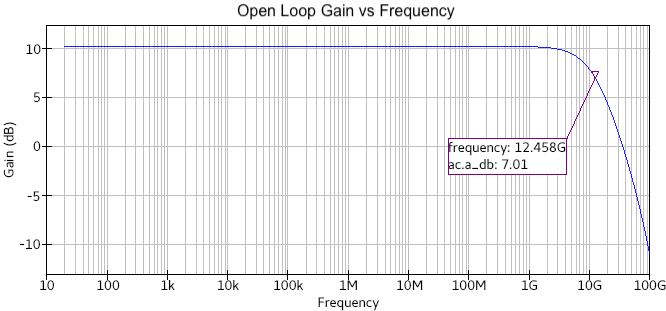
\includegraphics[width=.48\linewidth]{figure-4.png}\hfill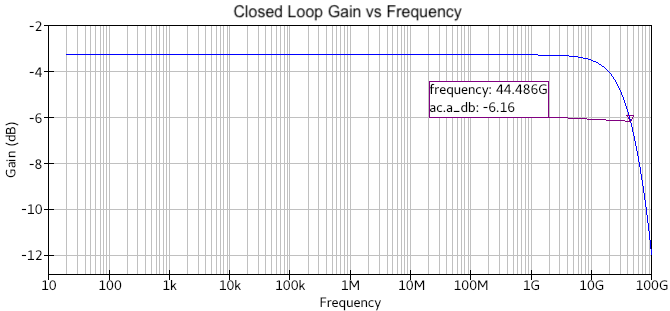
\includegraphics[width=.48\linewidth]{figure-5.png}
\caption{Open and closed loop Gain (dB) plotted against frequency. Frequency is plotted logarithmically ranging from 20 Hz to 100 GHz. The marker indicates a value used to interpolate the bandwidth.}
\label{fig:gain-responses}\end{figure}

\subsection{Low-Frequency Small-Signal Parameters}

From Equation~\eqref{eq:transconductance}, ${g}_{m}$ can be found by measuring the slope using two markers about the ${V}_{DS}=\ {V}_{GS}=Q$ operating point on the ${I}_{DS},\ {V}_{GS}$ curve. 
From Equation~\eqref{eq:output-resistance}, ${r}_{o}$ can be found by similarly measuring the slope's inverse on the ${I}_{DS},\ {V}_{DS}$ curve about $Q$. 
These results are presented in Table~\ref{tab:small-signal-parameters}.

\begin{table}[H]\centering
\begin{tabular}{lrr}\toprule
 & ${r}_{o}$ ($\Omega$) & ${g}_{m}$ ($\mathrm{mS}$) \\\midrule
NMOS & 500 & 13.3 \\
PMOS & 500 & 11.0 \\\bottomrule
\end{tabular}
\caption{Small-signal parameters extracted from the DC output and transfer characteristics of the NSCL-provided NMOS and PMOS components operating with the same parameters as $Q_1$ from Table~\ref{tab:fixed-design-values} and $Q_3$ from Table~\ref{tab:final-design}.}
\label{tab:small-signal-parameters}
\end{table}

\section{Discussion}

\subsection{DC Operating Point and Sizing}

The current-steering network scaled the $1\,\mathrm{mA}$ reference current using the nanowire ratios. For $NW_7=380$ and $NW_6=20$, Equation~\eqref{eq:current-mirror-scaling} predicts
\begin{equation}
    I_{D7}\approx 1\,\mathrm{mA}\frac{380}{20}=19\,\mathrm{mA}.
\end{equation}
The matched differential pair should therefore carry approximately $9.5\,\mathrm{mA}$ per branch, which is close to the simulated $9.84\,\mathrm{mA}$ through $Q_1$--$Q_4$. 
Since $Q_8$ supplies only the output branch, its required current and $NW_8$ are smaller than those of $Q_7$. The exact current ratios differ from the ideal width scaling because Equation~\eqref{eq:current-mirror-scaling} assumes equal drain-source voltages and neglects other short-channel effects.

The current steering network sets the currents $I_{D1}=I_{D2}=I_{D3}=I_{D4}$ as seen in Table~\ref{tab:final-design}. As a result, when increasing $NW_3$ and $NW_4$ while maintaining the same $I_D$, $V_{SG}$ must decrease for each PMOS by Equation~\eqref{eq:mosfet-current}.
Since $V_{S3} = V_{DD}$ is fixed, $V_{G3} = V_{D3}$ must increase. Therefore $V_{SD3}$ decreases when increasing $NW_3$, and $V_{DS1}$ increases. This opposing change allows us to tune the drain-source voltages for $Q_1$ to $Q_4$.

Similarly, $Q_5$'s drain current is set by $Q_8$. Increasing $NW_5$ reduces the $V_{GS5}$ required to maintain the same drain current. Since $V_{G5}$ is set by the current-mirror load, $V_{S5}=v_o$ therefore increases. This allows us to tune the output voltage. The final value of $v_o=0.225\,\mathrm{mV}$ is a small non-ideality because an ideal amplifier would produce zero output for equal input voltages.
\subsection{Gain and Feedback Performance}

The finite open-loop gain can be estimated from the measured small-signal parameters. 
Using Equation~\eqref{eq:first-stage-gain},
\begin{equation}
    A_{v1}\approx 13.3\,\mathrm{mS}
    \left(500\,\Omega\parallel500\,\Omega\right)
    =3.33,
\end{equation}
which corresponds to $10.4\,\mathrm{dB}$. 
This is close to the simulated open-loop gain of $10.2\,\mathrm{dB}$. 
The small difference is consistent with the source-follower gain being below unity and with the approximations made in the small-signal model. 
The finite values of $r_{o2}$ and $r_{o4}$ therefore limited the voltage gain compared with an ideal op-amp.
As discussed in Section 2.3.4, the output resistance is small but non-zero, unlike that of an ideal op-amp. Therefore, different loads which draw different currents will affect the voltage delivered to the load. 

The open-loop gain could be increased by reducing $I_{D7}$, which would reduce the currents through $Q_1$--$Q_4$. For fixed transistor sizes, Equation~\eqref{eq:intrinsic-gain-current} shows that $g_mr_o\propto1/\sqrt{I_D}$. 
Although reducing the drain current decreases $g_m$, it increases $r_o$ more strongly and therefore increases the intrinsic voltage gain. This would, however, move the drain currents away from the specified $10\,\mathrm{mA}$ operating condition.
Additionally, increasing $NW_1$ and $NW_2$ could increase $g_m$ and therefore increase the OL gain, although the resulting operating point would need to be retuned.

Using Equation~\eqref{eq:closed-loop-gain} and the experimental open-loop gain,
\begin{equation}
    A_{CL} = \frac{3.24}{1 + 3.24}
    =0.764,
\end{equation}

which corresponds to $-2.34\,\mathrm{dB}$, compared with the simulated $-3.27\,\mathrm{dB}$. Equation~\eqref{eq:closed-loop-gain} represents the amplifier as an ideal voltage-gain block, while the transistor circuit contains finite output resistances and a non-ideal source follower. The prediction therefore follows the simulated trend but does not give the exact closed-loop gain. Negative feedback still makes the response more closely resemble an ideal voltage follower by driving $v_o$ towards $v_i^+$.

The parasitic capacitances in the MOSFET models caused the gain to decrease at high frequencies, producing a finite bandwidth instead of the infinite bandwidth of an ideal op-amp. 
In the CL configuration, any change in $v_o$ also changes the inverting input voltage and therefore opposes the original change. 
This negative feedback makes the closed-loop response less sensitive to the reduction in open-loop gain with frequency. 
Consequently, the gain decreased from $10.2\,\mathrm{dB}$ in OL to $-3.27\,\mathrm{dB}$ in CL, while the bandwidth increased from $11.93\,\mathrm{GHz}$ to $45.57\,\mathrm{GHz}$.
Additionally, these parasitic capacitances lower impedance at higher frequencies. As a result, the input impedance deviates further from the ideal infinite input impedance at high frequencies.


\section{Conclusion}

Through iterative DC analysis, we successfully tuned $NW$ parameters to establish specified currents from a current steering network, equal drain-source voltages across a differential input and current mirror load, and reduced output offset voltage. 
AC testbenches produced an $A_{OL}=10.2\,\mathrm{dB}$, much smaller than that of the ideal op-amp due to the MOSFETs' finite output resistances and finite transconductance determined by device geometry and operating points. Similarly, $A_{CL}=-3.27\,\mathrm{dB}$ also differed from the ideal $0\,\mathrm{dB}$.
Due to parasitic capacitances, the bandwidths of both the OL and CL amplifiers are finite.

\begin{thebibliography}{9}
\bibitem{qucs}
Qucs-S Project, ``Qucs-S: A Qucs GUI for SPICE simulators.''
\url{https://ra3xdh.github.io/}

\bibitem{brief}
\emph{Simulation Project: ETIN71 -- Introduction to Integrated Electronics}, Lund University, 2026.
\end{thebibliography}

\end{document}
